\begin{figure}[htbp]
\section*{PTPN11}
\centering
\begin{subfigure}[b]{0.95\textwidth}
\centering
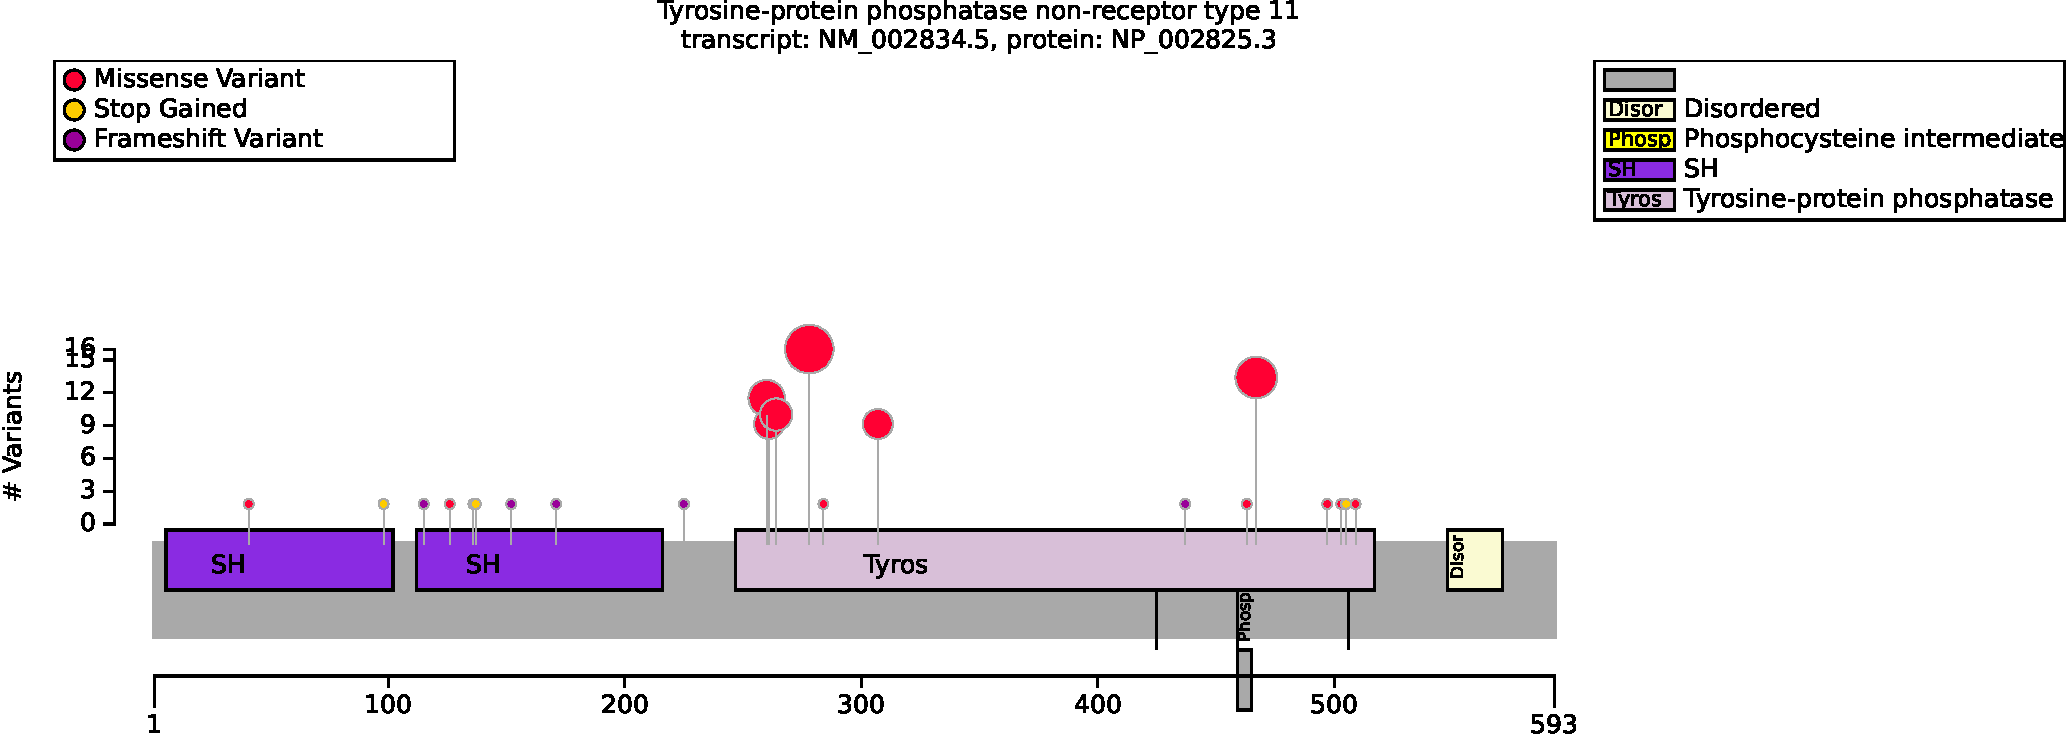
\includegraphics[width=\textwidth]{ img/PTPN11_protein_diagram.pdf} 
\captionsetup{justification=raggedright,singlelinecheck=false}
\caption{Distribution of variants in PTPN11}
\end{subfigure}

\vspace{2em}

\begin{subfigure}[b]{0.95\textwidth}
\centering
\resizebox{\textwidth}{!}{
\begin{tabular}{llllrr}
\toprule
HPO term & Missense & Other & p-value & adj. p-value\\
\midrule
Hypertelorism [HP:0000316] & 37/41 (90\%) & 0/12 (0\%) & $6.82\times 10^{-9}$ & $2.73\times 10^{-8}$\\
Intellectual disability, mild [HP:0001256] & 8/23 (35\%) & 0/12 (0\%) & 0.032 & 0.032\\
Pulmonic stenosis [HP:0001642] & 18/34 (53\%) & 0/12 (0\%) & 0.001 & 0.002\\
Webbed neck [HP:0000465] & 15/20 (75\%) & 0/12 (0\%) & $2.94\times 10^{-5}$ & $5.88\times 10^{-5}$\\
\bottomrule
\end{tabular}
}
\captionsetup{justification=raggedright,singlelinecheck=false}
\caption{Fisher Exact Test performed to compare HPO annotation frequency with respect to Missense and Other. Total of 4 tests were performed.}
\end{subfigure}
\vspace{2em}
\begin{subfigure}[b]{0.95\textwidth}
\centering
\resizebox{\textwidth}{!}{
\begin{tabular}{llllrr}
\toprule
Genotype (A) & Genotype (B) & total tests performed & significant results\\
\midrule
Tyr279Cys & Other & 8 & 0\\
TK domain N term & TK domain C term & 5 & 0\\
FEMALE & MALE & 6 & 0\\
\bottomrule
\end{tabular}
}
\captionsetup{justification=raggedright,singlelinecheck=false}
\caption{Fisher Exact Test performed to compare HPO annotation frequency with respect to genotypes.}
\end{subfigure}

\vspace{2em}

\caption{The cohort comprised 70 individuals (27 females, 33 males, 10 with unknown sex). A total of 69 HPO terms were used to annotate the cohort. Disease diagnoses: LEOPARD syndrome 1 (OMIM:151100) (31 individuals), Noonan syndrome 1 (OMIM:163950) (27 individuals), Metachondromatosis (OMIM:156250) (12 individuals). No previous statistical analysis of correlations with PTPN11 missense variants was identified in the medical literature. A total of 27 unique variant alleles were found in \textit{PTPN11} (transcript: \texttt{NM\_002834.5}, protein id: \texttt{NP\_002825.3}).}
\end{figure}
